\subsection{Estación Terminal}

Las estaciones terminales presentan una gran cantidad de vías principales y plataformas en paralelo, en las cuales confluyen una o varias líneas ferroviarias. A diferencia de estaciones de alta densidad que pueden presentar finales de vía relativos, las estaciones terminales poseen finales de vía absolutos. Es decir, las formaciones que circulan por la vía descendente deberán detener su marcha completamente antes de llegar al fía de vía, para luego retomar su marcha en sentido contrario, por la vía ascendente. Esta operación puede realizarse de manera inmediata en formaciones con locomotras eléctricas en ambos extremos del tren o con locomotoras diesel luego de varias maniobras que requieren el uso de diversos cambios de vías. En la Figura \ref{fig:terminal_1} se ilustra un ejemplo de una estación terminal.

    \begin{figure}[H]
        \centering
        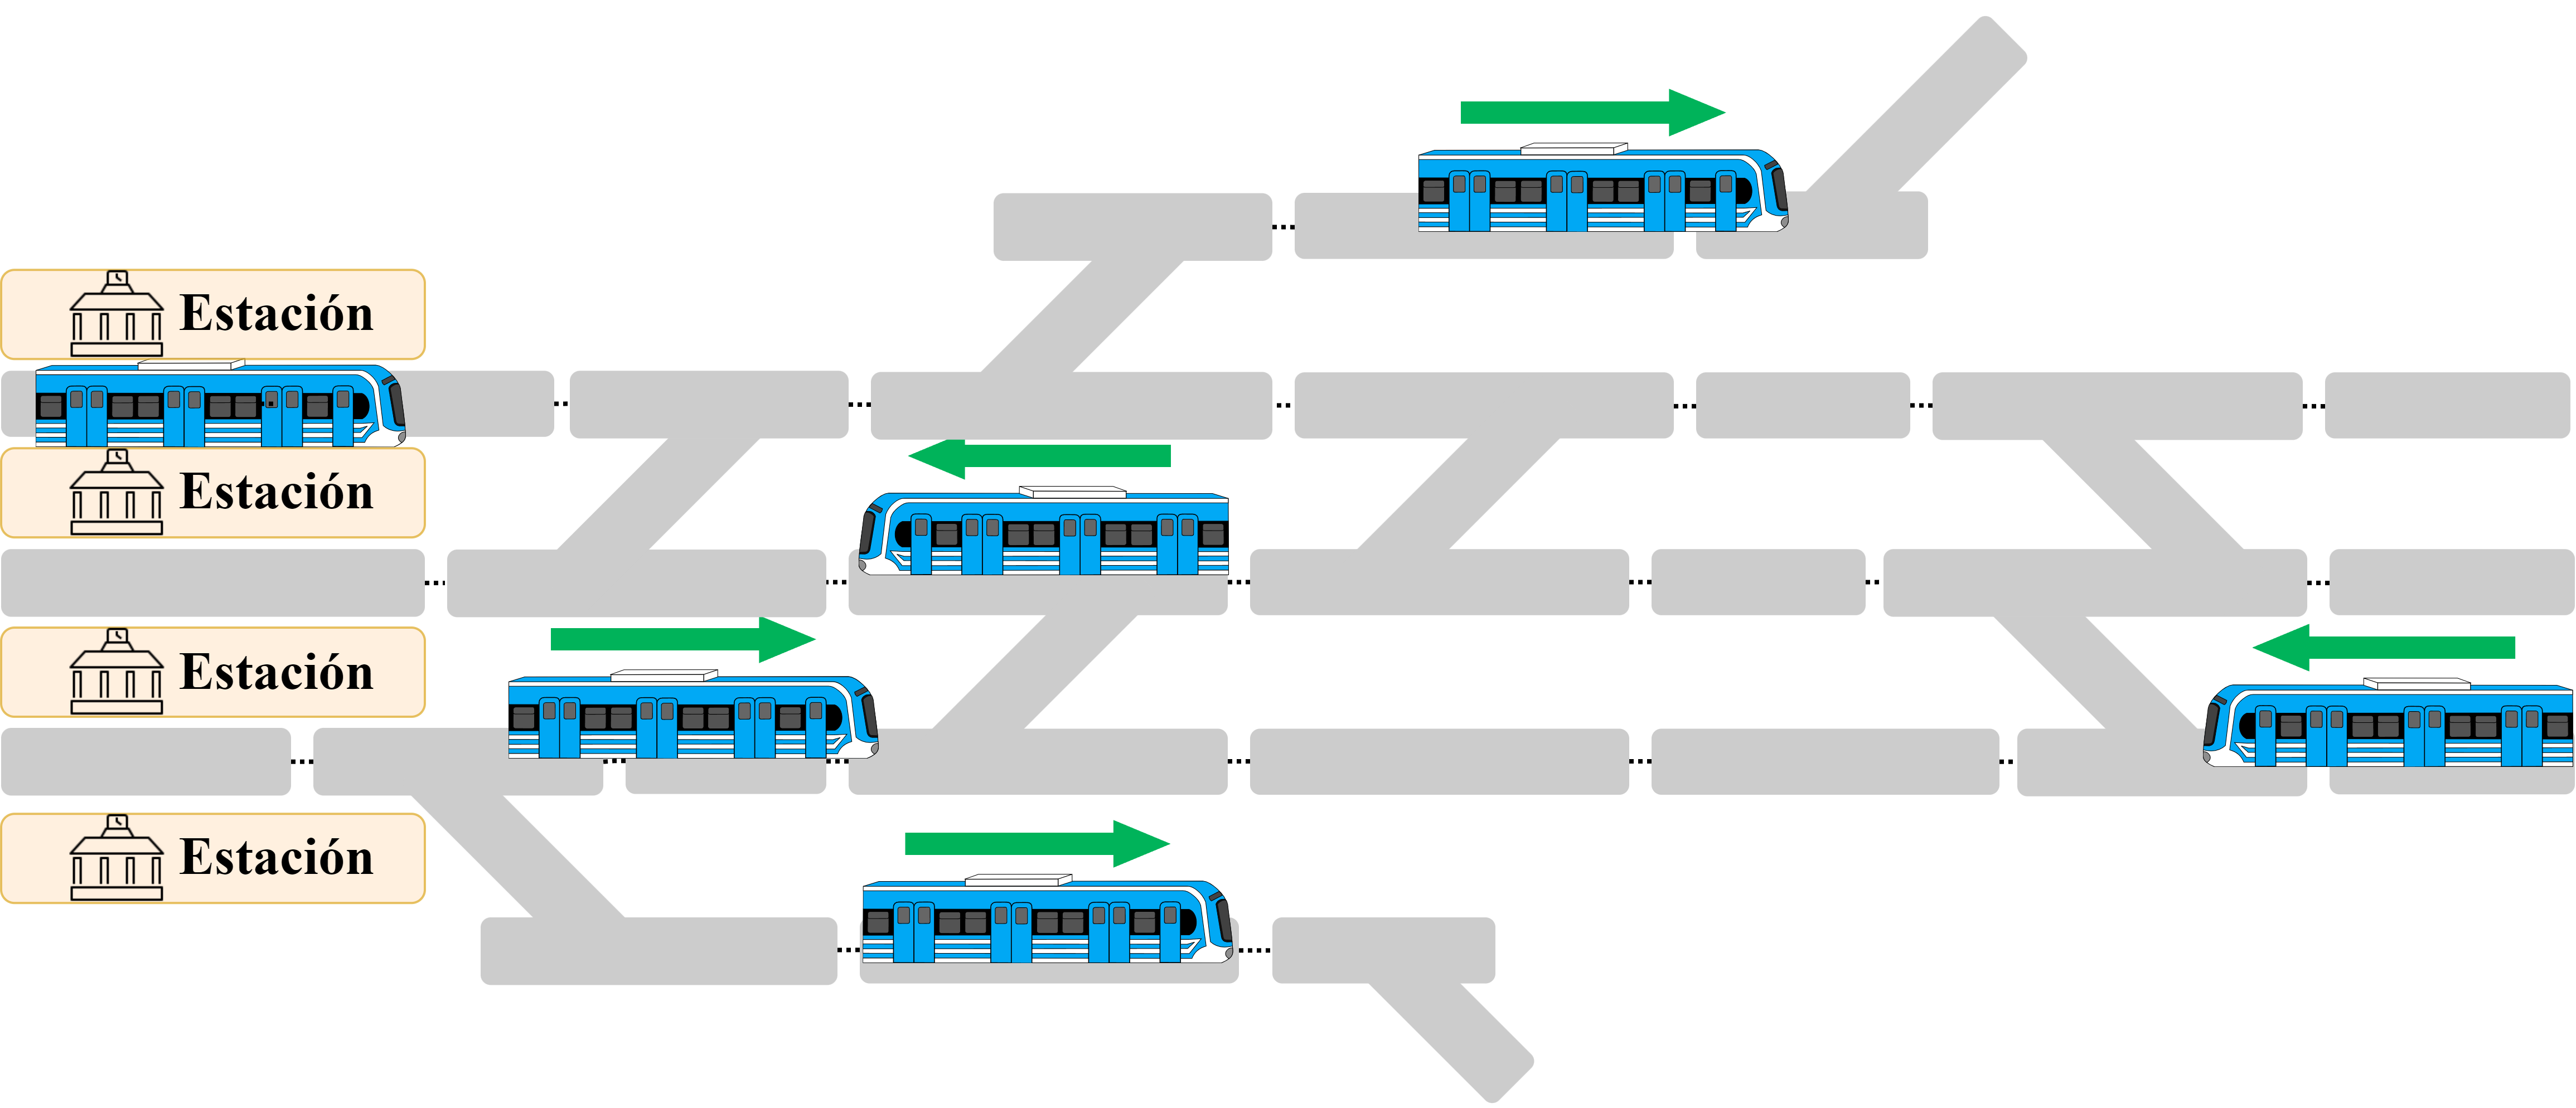
\includegraphics[width=1\textwidth]{Figuras/terminal}
        \centering\caption{Topología terminal.}
        \label{fig:terminal_1}
    \end{figure}

En las estaciones terminales suelen confluir la información en tiempo real de la terminal y las estaciones más próximas de la línea, o incluso la información en tiempo real de la totalidad de la línea. Esta característica, además de ser la estación de mayor tamaño de la línea, les otorga una jerarquía tal que suelen concentrar parcial o totalmente el control del señalamiento de la red. Las decisiones tomadas en una estación terminal tienen un gran impacto en el sistema de transporte de toda la línea, directa o indirectamente. Estas operaciones deben considerar cientos o miles de estados en simultáneo, por lo que ejecutarlas de forma manual es muy complejo o incluso imposible. Un sistema de enclavamientos moderno, robusto, que pueda garantizar una altísima disponibilidad, mantenibilidad y seguridad es indispensable para llevar a cabo estas tareas.